\section{Modelos}

\subsection{Comparación visual de los árboles}
El ajuste mediante \texttt{GridSearch} produce un árbol más \textbf{compacto} y, por tanto, \textbf{más explicable} (menos profundidad y reglas), manteniendo o mejorando ligeramente la precisión respecto al baseline. A continuación se muestran por separado ambos diagramas con la misma profundidad visualizada para facilitar la lectura.

\begin{figure}[h]
  \centering
  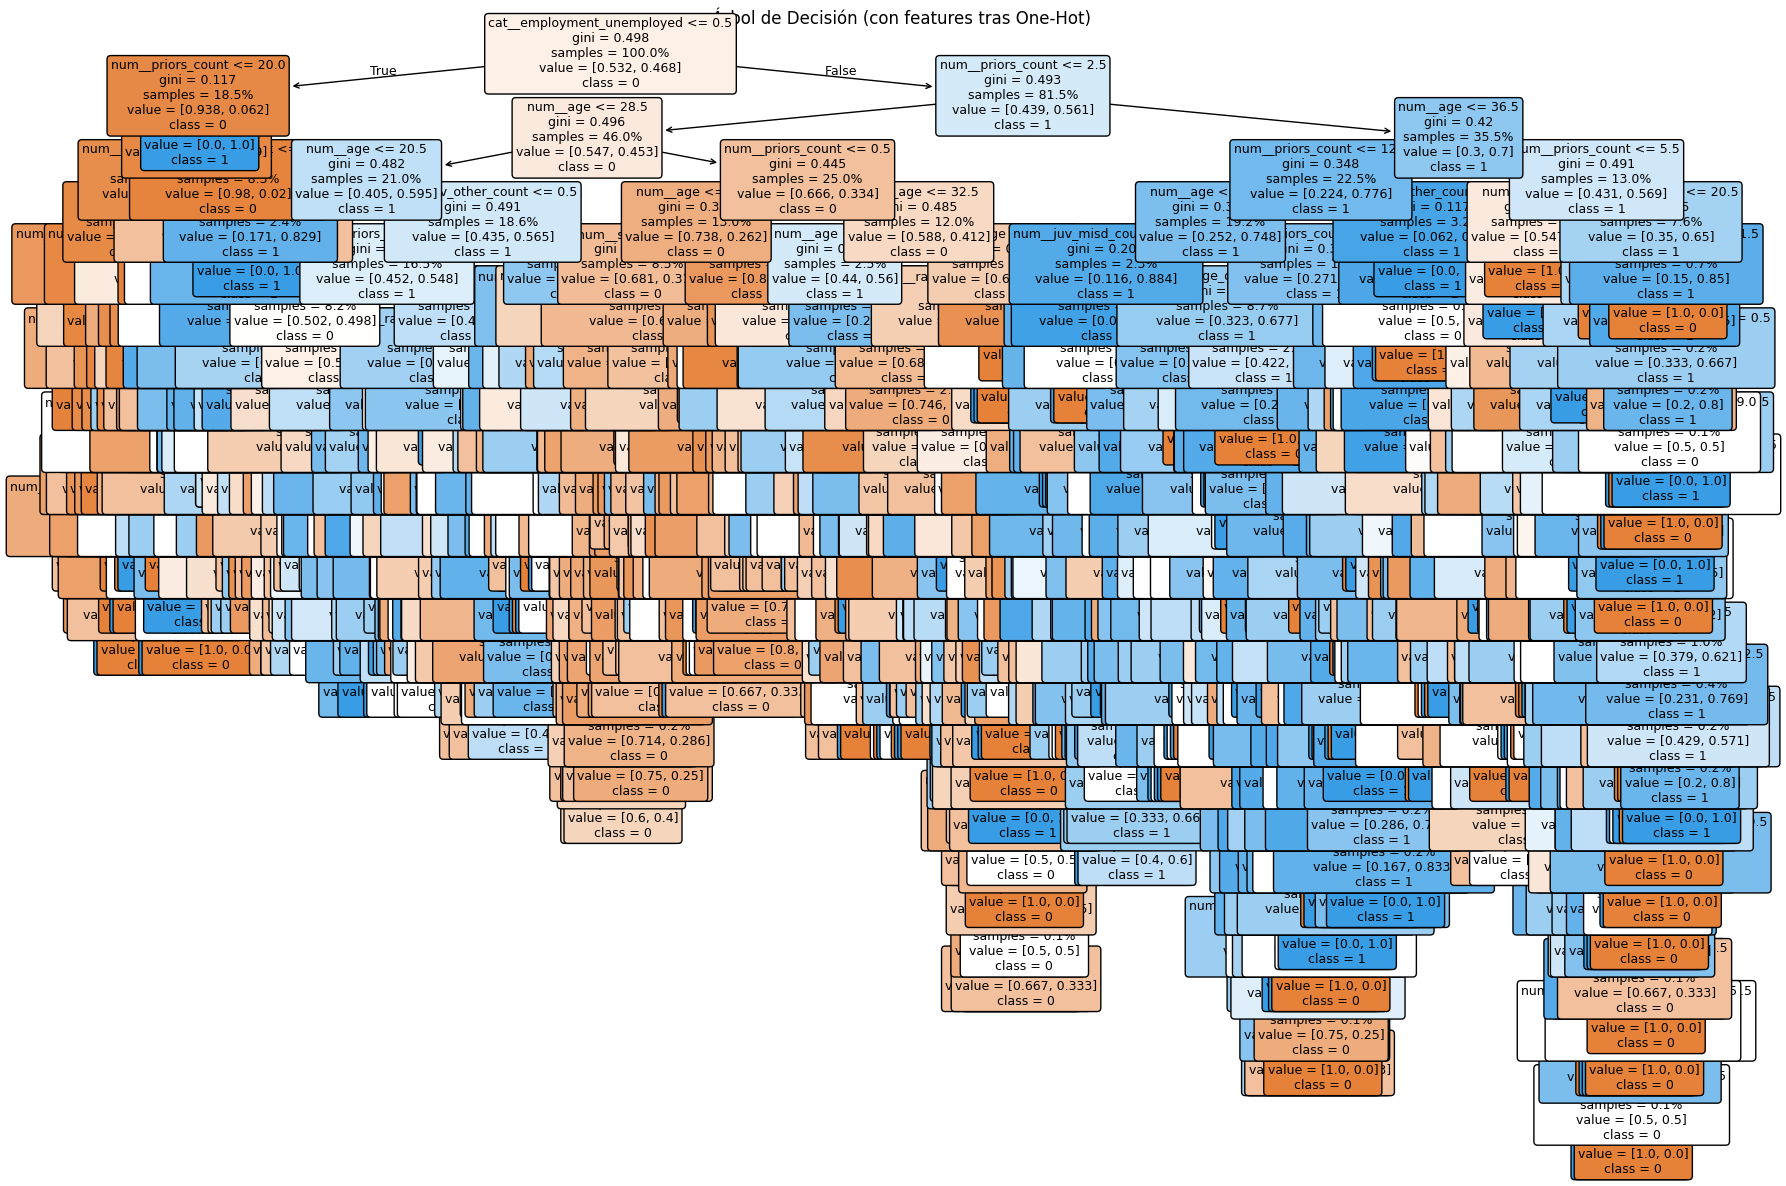
\includegraphics[width=0.92\linewidth]{figures/decision_tree_baseline_depth.png}
  \caption{Decision Tree (baseline), profundidad visualizada = 3.}
  \label{fig:tree-base}
\end{figure}

\begin{figure}[h]
  \centering
  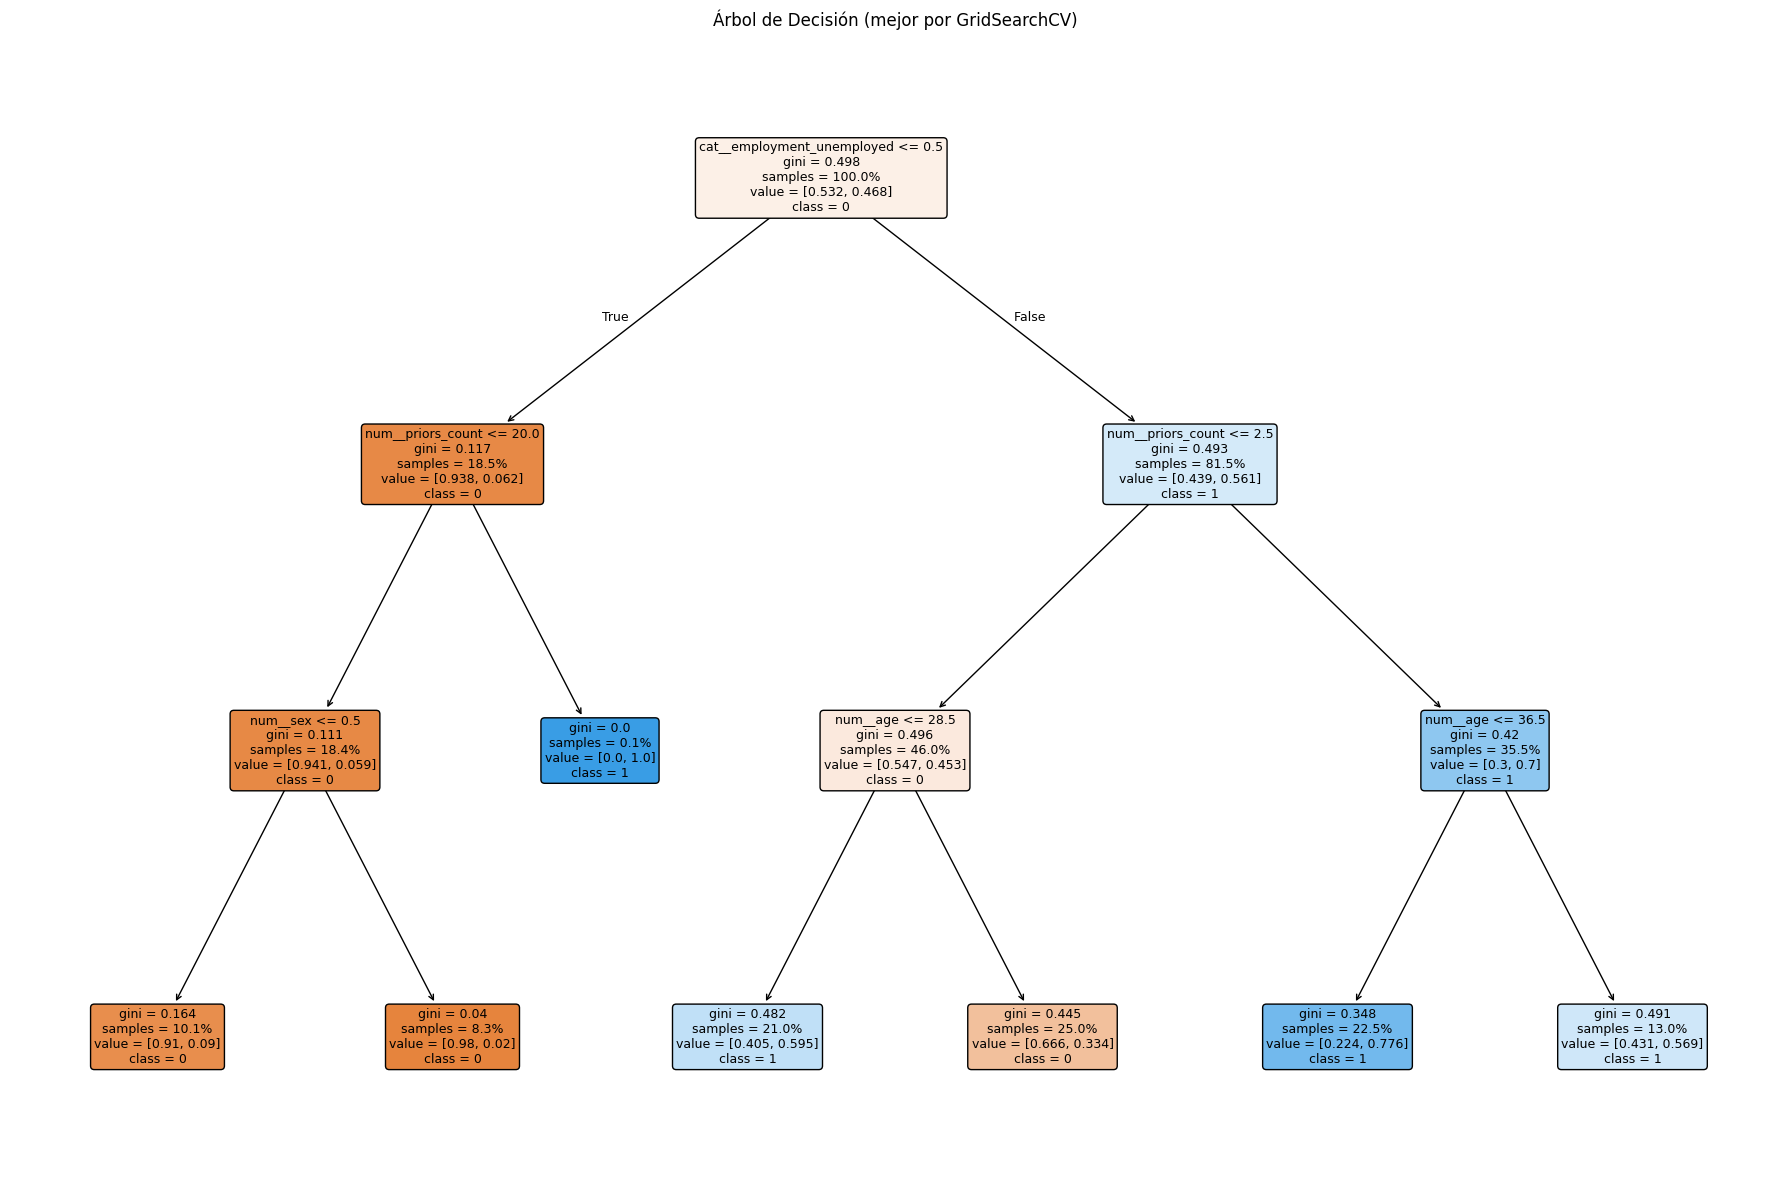
\includegraphics[width=0.92\linewidth]{figures/decision_tree_tunned_depth.png}
  \caption{Decision Tree (tuned), profundidad visualizada = 3.}
  \label{fig:tree-tuned}
\end{figure}


\begin{figure}[h]
  \centering
  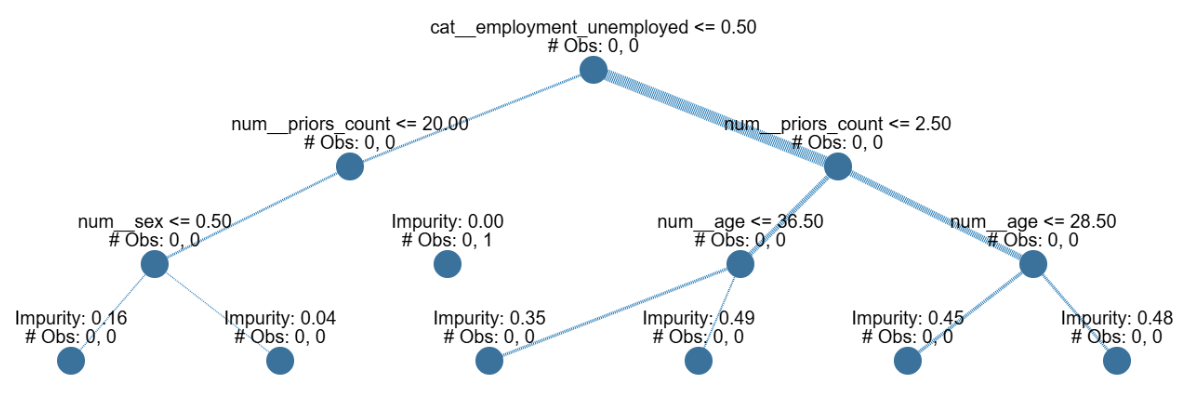
\includegraphics[width=0.92\linewidth]{figures/decision_tree_tunned_depth_global.png}
  \caption{Decision Tree (tuned) global con librería \textit{interpret}.}
  \label{fig:tree-tuned_global}
\end{figure}








\subsection{Explicación global}

El árbol ajustado concentra la decisión en pocas divisiones y umbrales sencillos, lo que facilita su lectura y comunicación. En la raíz aparece \texttt{employment\_unemployed}; a partir de ahí, \texttt{num\_priors\_count} y \texttt{age} modulan la predicción con cortes aproximados que se repiten en las ramas principales.

\paragraph{Tendencias clave.}
\begin{itemize}
  \item \textbf{Situación laboral}: si no está desempleado ($\leq 0.5$) la predicción suele inclinarse a clase 0; si está desempleado ($> 0.5$), el pronóstico depende sobre todo de antecedentes y edad.
  \item \textbf{Antecedentes} (\texttt{num\_priors\_count}): en personas empleadas, valores altos ($>20$) llevan a clase 1; en desempleados, el corte relevante baja (en torno a $2.5$).
  \item \textbf{Edad} (\texttt{age}): con pocos antecedentes, $\leq 28.5$ empuja a clase 1 y $>28.5$ a clase 0; con más antecedentes, incluso mayores de $\sim 36.5$ pueden seguir en clase 1.
  \item \textbf{Sexo}: aporta poco y solo ajusta la pureza en subramas concretas.
\end{itemize}

\paragraph{Reglas representativas (modelo ajustado).}
\vspace{-0.4em}
\begin{itemize}
  \item R1: \texttt{employment\_unemployed} $\leq 0.5$ $\land$ \texttt{num\_priors\_count} $\leq 20$ $\Rightarrow$ clase 0.
  \item R2: \texttt{employment\_unemployed} $\leq 0.5$ $\land$ \texttt{num\_priors\_count} $> 20$ $\Rightarrow$ clase 1.
  \item R3: \texttt{employment\_unemployed} $> 0.5$ $\land$ \texttt{num\_priors\_count} $\leq 2.5$: 
        si \texttt{age} $\leq 28.5$ $\Rightarrow$ clase 1; si \texttt{age} $> 28.5$ $\Rightarrow$ clase 0.
  \item R4: \texttt{employment\_unemployed} $> 0.5$ $\land$ \texttt{num\_priors\_count} $> 2.5$: 
        si \texttt{age} $\leq 36.5$ $\Rightarrow$ clase 1; si $> 36.5$ $\Rightarrow$ clase 1 (con menor pureza).
\end{itemize}

\paragraph{Comentario.}
El \texttt{GridSearch} no solo mejora ligeramente las métricas frente al baseline, sino que produce un árbol más \emph{compacto}: menos profundidad y menos reglas, por lo que se puede representar y recorrer con claridad.

% =======================
% Caso 0 — Falso positivo
% =======================
\paragraph{Explicación local (Caso 0 — Falso positivo)}.

\begin{figure}[h!]
  \centering
  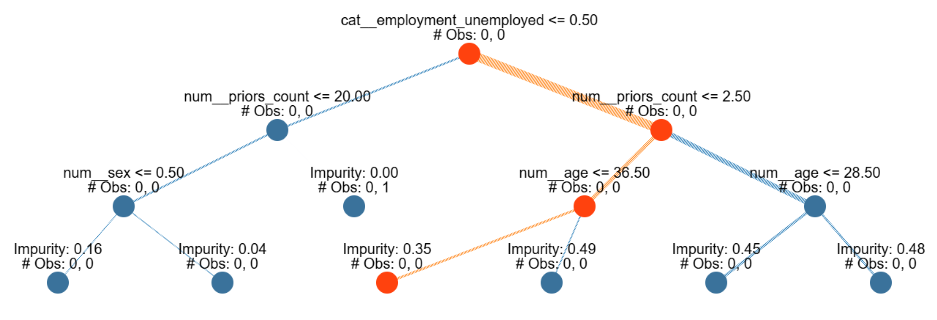
\includegraphics[width=0.92\linewidth]{figures/decision_tree_tunned_depth_local0.png}
  \caption{Decision Tree (tuned) local caso 0 con librería \textit{interpret}.}
  \label{fig:tree-tuned_local0}
\end{figure}

% --- Predicción y hoja alcanzada ---
\begin{table}[h!]
\centering
\caption{Predicción del modelo para el Caso 0.}
\label{tab:local-pred-caso0}
\small
\begin{tabular}{@{}lccc@{}}
\toprule
\textbf{Clase real} & \textbf{Clase predicha} & \textbf{PrScore} & \textbf{Decisión} \\
\midrule
0 & 1 & 0.776 & Falso positivo \\
\bottomrule
\end{tabular}
\end{table}

% --- Ruta de decisión (condiciones) ---
\begin{table}[h!]
\centering
\caption{Ruta de decisión seguida (Caso 0).}
\label{tab:local-path-caso0}
\small
\begin{tabular}{@{}cll@{}}
\toprule
\# & \textbf{Condición en el nodo} & \textbf{Rama} \\
\midrule
1 & \texttt{employment\_\_unemployed} \(> 0.5\) & Derecha \\
2 & \texttt{num\_\_priors\_count} \(\le 2.5\)   & Izquierda \\
3 & \texttt{num\_\_age} \(\le 36.5\)            & Hoja clase 1 \\
\bottomrule
\end{tabular}
\end{table}

El modelo considera que \texttt{desempleo + pocos antecedentes + edad ≤ 36.5} implica riesgo (clase 1). Sin embargo, se equivoca, pues la clase real era 0. La confianza es relativamente alta (0.776).

% =======================
% Caso 1 — Verdadero negativo
% =======================
\paragraph{Explicación local (Caso 1 — Verdadero negativo)}.

\begin{figure}[h!]
  \centering
  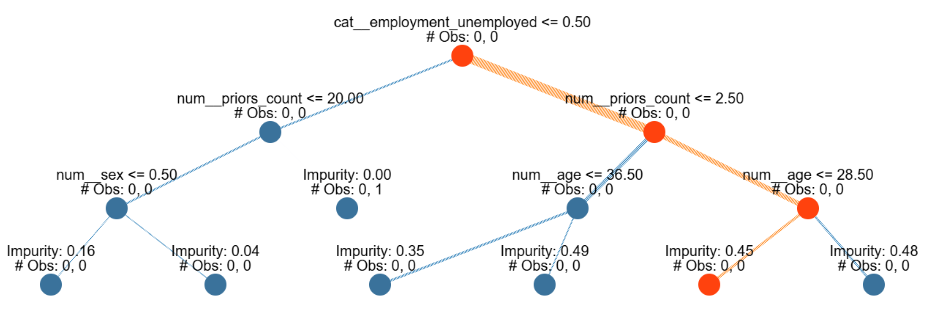
\includegraphics[width=0.92\linewidth]{figures/decision_tree_tunned_depth_local1.png}
  \caption{Decision Tree (tuned) local caso 1 con librería \textit{interpret}.}
  \label{fig:tree-tuned_local1}
\end{figure}

\begin{table}[h!]
\centering
\caption{Predicción del modelo para el Caso 1.}
\label{tab:local-pred-caso1}
\small
\begin{tabular}{@{}lccc@{}}
\toprule
\textbf{Clase real} & \textbf{Clase predicha} & \textbf{PrScore} & \textbf{Decisión} \\
\midrule
0 & 0 & 0.666 & Verdadero negativo \\
\bottomrule
\end{tabular}
\end{table}

\begin{table}[h!]
\centering
\caption{Ruta de decisión seguida (Caso 1).}
\label{tab:local-path-caso1}
\small
\begin{tabular}{@{}cll@{}}
\toprule
\# & \textbf{Condición en el nodo} & \textbf{Rama} \\
\midrule
1 & \texttt{employment\_\_unemployed} \(> 0.5\) & Derecha \\
2 & \texttt{num\_\_priors\_count} \(\le 2.5\)   & Izquierda \\
3 & \texttt{num\_\_age} \(\le 28.5\)            & Hoja clase 0 \\
\bottomrule
\end{tabular}
\end{table}

En el subgrupo de desempleados con pocos antecedentes, la condición de ser muy joven (≤ 28.5) lleva al modelo a predecir bajo riesgo (clase 0), en este caso de forma correcta.

% =======================
% Caso 2 — Verdadero positivo
% =======================
\paragraph{Explicación local (Caso 2 — Verdadero positivo)}.

\begin{figure}[h!]
  \centering
  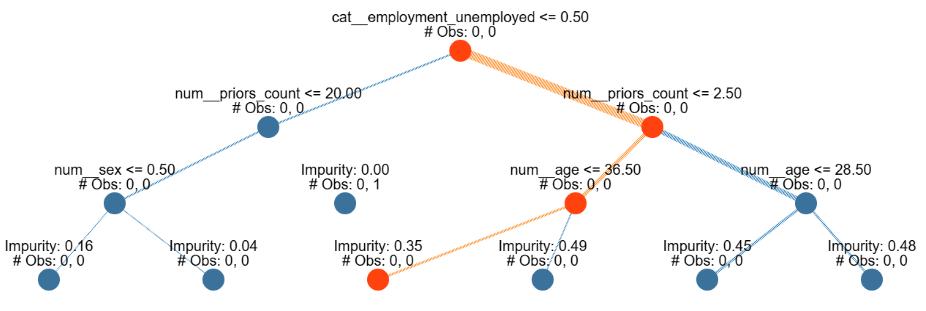
\includegraphics[width=0.92\linewidth]{figures/decision_tree_tunned_depth_local2.png}
  \caption{Decision Tree (tuned) local caso 2 con librería \textit{interpret}.}
  \label{fig:tree-tuned_local2}
\end{figure}

\begin{table}[h!]
\centering
\caption{Predicción del modelo para el Caso 2.}
\label{tab:local-pred-caso2}
\small
\begin{tabular}{@{}lccc@{}}
\toprule
\textbf{Clase real} & \textbf{Clase predicha} & \textbf{PrScore} & \textbf{Decisión} \\
\midrule
1 & 1 & 0.776 & Verdadero positivo \\
\bottomrule
\end{tabular}
\end{table}

\begin{table}[h!]
\centering
\caption{Ruta de decisión seguida (Caso 2).}
\label{tab:local-path-caso2}
\small
\begin{tabular}{@{}cll@{}}
\toprule
\# & \textbf{Condición en el nodo} & \textbf{Rama} \\
\midrule
1 & \texttt{employment\_\_unemployed} \(> 0.5\) & Derecha \\
2 & \texttt{num\_\_priors\_count} \(\le 2.5\)   & Izquierda \\
3 & \texttt{num\_\_age} \(\le 36.5\)            & Hoja clase 1 \\
\bottomrule
\end{tabular}
\end{table}

Mismo patrón que el Caso 0 (\texttt{desempleo + juventud relativa}), pero aquí acierta al asignar riesgo (clase 1).

% =======================
% Caso 3 — Falso negativo
% =======================
\paragraph{Explicación local (Caso 3 — Falso negativo)}.

\begin{figure}[h!]
  \centering
  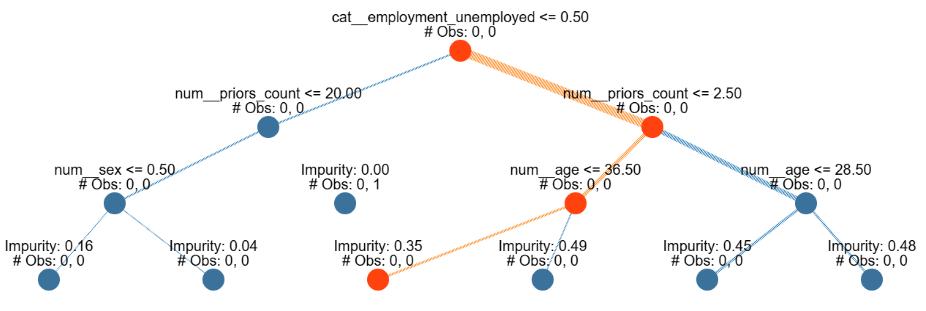
\includegraphics[width=0.92\linewidth]{figures/decision_tree_tunned_depth_local2.png}
  \caption{Decision Tree (tuned) local caso 3 con librería \textit{interpret}.}
  \label{fig:tree-tuned_local3}
\end{figure}

\begin{table}[h!]
\centering
\caption{Predicción del modelo para el Caso 3.}
\label{tab:local-pred-caso3}
\small
\begin{tabular}{@{}lccc@{}}
\toprule
\textbf{Clase real} & \textbf{Clase predicha} & \textbf{PrScore} & \textbf{Decisión} \\
\midrule
1 & 0 & 0.666 & Falso negativo \\
\bottomrule
\end{tabular}
\end{table}

\begin{table}[h!]
\centering
\caption{Ruta de decisión seguida (Caso 3).}
\label{tab:local-path-caso3}
\small
\begin{tabular}{@{}cll@{}}
\toprule
\# & \textbf{Condición en el nodo} & \textbf{Rama} \\
\midrule
1 & \texttt{employment\_\_unemployed} \(> 0.5\) & Derecha \\
2 & \texttt{num\_\_priors\_count} \(\le 2.5\)   & Izquierda \\
3 & \texttt{num\_\_age} \(\le 28.5\)            & Hoja clase 0 \\
\bottomrule
\end{tabular}
\end{table}

La misma subregla que el Caso 1 (joven, pocos antecedentes, desempleado) lleva a clasificar como bajo riesgo, pero en este caso el individuo sí era de clase 1. Se observa una tendencia del árbol a subestimar riesgo en este perfil.

% =======================
% Caso 4 — Verdadero negativo
% =======================
\paragraph{Explicación local (Caso 4 — Verdadero negativo)}.

\begin{table}[h!]
\centering
\caption{Predicción del modelo para el Caso 4.}
\label{tab:local-pred-caso4}
\small
\begin{tabular}{@{}lccc@{}}
\toprule
\textbf{Clase real} & \textbf{Clase predicha} & \textbf{PrScore} & \textbf{Decisión} \\
\midrule
0 & 0 & 0.666 & Verdadero negativo \\
\bottomrule
\end{tabular}
\end{table}

\begin{table}[h!]
\centering
\caption{Ruta de decisión seguida (Caso 4).}
\label{tab:local-path-caso4}
\small
\begin{tabular}{@{}cll@{}}
\toprule
\# & \textbf{Condición en el nodo} & \textbf{Rama} \\
\midrule
1 & \texttt{employment\_\_unemployed} \(> 0.5\) & Derecha \\
2 & \texttt{num\_\_priors\_count} \(\le 2.5\)   & Izquierda \\
3 & \texttt{num\_\_age} \(\le 28.5\)            & Hoja clase 0 \\
\bottomrule
\end{tabular}
\end{table}

\begin{figure}[h!]
  \centering
  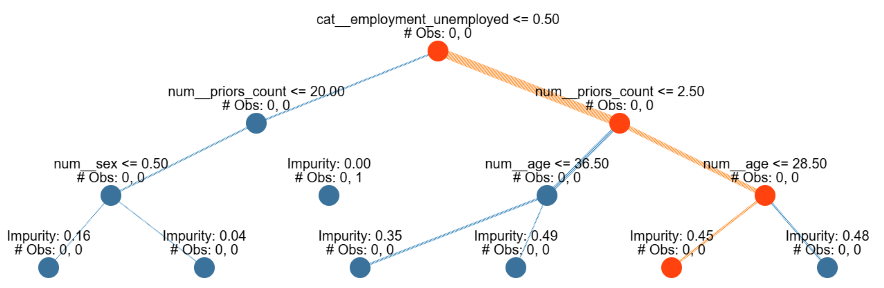
\includegraphics[width=0.92\linewidth]{figures/decision_tree_tunned_depth_local4.png}
  \caption{Decision Tree (tuned) local caso 4 con librería \textit{interpret}.}
  \label{fig:tree-tuned_local4}
\end{figure}

El patrón “desempleado, pocos antecedentes, edad baja” vuelve a dar clase 0, esta vez de forma correcta.

